\chapter{Subgame-Margin Maximization}
\label{ch:max-margin}
\epigraphLong{
  I have discovered a~truly marvellous proof of~this, which this margin is too narrow to contain.
}{Pierre de Fermat on \emph{Fermat's Last Theorem}}
\vskip -2em
\note{
  This chapter summarizes our own paper~(\cite{Moravcik2016refining}).
}

\section{Motivation and Overview}
The outline of~this chapter is:
\begin{enumerate}[(1)]
    \setlength\itemsep{-.5ex}
  \item listing the steps used by~our technique,
  \item using the problem of~refining imperfect-information subgames to motivate a~value to be maximized,
  \item formalizing this value as the \emph{\acrlong{sm}},
  \item discuss and formalize its properties,
  \item formulate an~\acrshort{lp} optimizing the \acrshort{sm},
  \item describe a~corresponding \acrshort{efg} construction: \emph{a~max-margin gadget}.
\end{enumerate}
Our technique follows the steps of~the subgame-refinement framework:
\begin{enumerate}[(i)]
    \setlength\itemsep{-.5ex}
  \item create an~abstraction for the game;
  \item compute an~equilibrium approximation within the abstraction,
  \item play according to this strategy,
  \item when the play reaches final stage of~the game, create a~fine-grained abstraction for the endgame,
  \item refine the strategy in~the fine-grained abstraction,
  \item use the resulting strategy in that subgame (creating a~combined strategy).
\end{enumerate}
Since all the steps except for (v) are identical to already described techniques, we describe only step (v) in details.

\section{Subgame Margin}
\epigraph{
  Your margin is my opportunity.
}{Jeff Bezos}
To address the potential increase in~exploitability caused by an~opponent altering his behavior in the trunk, we ensure that there is no~distribution of~starting states that would allow him to increase his CBV when confronted by subgame refinement.
The simplest way to ensure this is to decrease his CBV in~all possible starting states.
We can put a~lower bound on~this improvement by measuring the state with the smallest decrease in CBV.
Our goal is to maximize this lower bound.
We refer to this values as the \acrfull{sm}.

\begin{defn}[\acrlong{sm}]
  Let $\sigma_1$, $\sigma_1'$ be a~pair of~player~$1$'s strategies for subgame~$S$.
  Then a~\acrlong{sm}
  \[
    SM_1 (\sigma_1, \sigma_1' , S) =
    \min_{I_2 \in \I_2^{R(S)}}
    \left( CBV_2^{\sigma_1} (I_2) - CBV_2^{\sigma_1'} (I_2) \right)
  \]
  measures the ``gap in~decrease'' between the old and the new \acrlong{cbv}s, across all root information sets $I_2 \in \I_2^{R(S)}$.
\end{defn}

Subgame margin has several useful properties.
The exploitability is strongly related to the value of~the margin:
if it is non-negative, the new combined strategy is guaranteed to be no more exploitable than the original one.
To prove it, we will first re-state Theorem~\ref{thm:cf-val-and-utility} using the following lemma:
\begin{lem}
  \label{lem:cbv-and-sm}
  $CBV_2^{\sigma_1'} (I_2) \leq CBV_2^{\sigma_1} (I_2)$ for all $I_2 \in \I_2^{R(S)}$
  iff
  $SM_1 (\sigma_1, \sigma_1' , S) \geq 0.$
\end{lem}
\begin{proof}
  $
  CBV_2^{\sigma_1'} (I_2) \leq CBV_2^{\sigma_1} (I_2)
  \quad \Longleftrightarrow \quad
  0 \leq CBV_2^{\sigma_1} (I_2) - CBV_2^{\sigma_1'} (I_2)
  \quad \Longleftrightarrow \quad
  0 \leq \min_{I_2 \in \I_2^{R(S)}} \left( CBV_2^{\sigma_1} (I_2) - CBV_2^{\sigma_1'} (I_2) \right)
  = SM_1 (\sigma_1, \sigma_1' , S)
  $
\end{proof}

\begin{cor}[Theorem~\ref{thm:cf-val-and-utility} via \acrlong{sm}]
  \label{cor:sm-and-utility}
  Given a~strategy~$\sigma_1$, a~subgame~$S$, and a~re-solved subgame strategy~$\sigma_1^S$, let $\sigma_1' = \sigma_{1, [S \leftarrow \sigma_1^S]}$ be the combination of~$\sigma_1$ and~$\sigma_1^S$.
  If $SM_1 (\sigma_1, \sigma_1' , S) \geq 0$, then $u_2(\sigma_1', \textrm{CBR}(\sigma_1')) \leq  u_2(\sigma_1, \textrm{CBR}(\sigma_1))$.
\end{cor}

Moreover, given that the opponent's best response reaches the subgame with non-zero probability, the exploitability of~our combined strategy is even reduced.
This improvement is at~least proportional to the subgame margin:

\begin{thm}[improvement proportional to the \acrlong{sm}]
  \label{thm:improvement-propto-sm}
  With the $S$, $\sigma_1$ and $\sigma_1'$ from the Corollary, also assume there exists a~\acrlong{br}~$\sigma_2^* = BR(\sigma_1')$ such that $\pi^{<\sigma_1',\sigma_2^*>} (I_2) > 0$ for some $I_2 \in\I_2^{R(S)}$.
  Then 
  \[
    u_1(\sigma_1', CBR(\sigma_1')) - u_1(\sigma_1, CBR(\sigma_1)) \ge \pi_{-2}^{\sigma_1'} (I_2) \cdot SM_1(\sigma_1, \sigma_1', S).
  \]
\end{thm}
\begin{proof}
  \todo
\end{proof}
Though this lower bound might seem artificial at~first, it has promising properties for the subgame refinement.
Since we refine the strategy once we reach the subgame, either we face $2$'s \acrlong{br} that reaches $S$, or he has made a~mistake earlier in the game.

Furthermore, the probability of~player~$1$ reaching a~subgame is proportional to $\pi_{-2}^{\sigma_1'}(I_2)$.
As this term (and by extension, the bound) grows, the probability of~reaching that subgame increases.
In conclusion, we are more likely to reach a~subgame with a~larger bound.

\section{Linear Program}
To formulate the subgame-margin maximization as an~\acrshort{lp}, we easily modify (\ref{lp:cfr-d}):
\begin{equation}
  \label{lp:max-margin}
  \begin{split}
    \max_{v, x}\ &\textcolor{red}{m} \\
    v_I - m &\ge CBV_2^\sigma(I), \quad I \in \I_2^{R(S)}\\ 
    Ex &= e \\
    F^\top v - A_2^\top x &\le \vect{0} \\
    x &\ge \vect{0},
  \end{split}
\end{equation}
where $m$ is a~scalar corresponding to the subgame margin that we aim to~maximize.
It serves as ``a gap'' between all values $v_I$ and the given constants $CBV_2^\sigma(I)$, and we wish to make this gap as~large as~possible.

The similarities between (\ref{lp:max-margin}) and (\ref{lp:cfr-d}) make it easier to see our improvement:
whereas the \acrshort{lp} (\ref{lp:cfr-d}) only guarantees a~non-negative margin, we maximize it.
Although the optimization formulation is almost identical to~the re-solving, our gadget construction is different.

\section{Equivalent Gadget Game}
\epigraphLong{
  A~new gadget that lasts only five minutes is worth more than an~immortal work that bores everyone.
}{Francis Picabia}
One way to find the refined strategy is to solve the corresponding \acrfull{lp}.
However, algorithms that are tailor-made for \acrshort{efg}s often outperform the optimization approach (\cite{Bosansky2013solving}).
These algorithms often permit the use of~domain-specific tricks to provide further performance gains (\cite{Johanson2012efficient}).
Thus, formulating our optimization problem~(\ref{lp:max-margin}) as an \acrshort{efg} will mean that we can compute larger subgame abstractions using the available computing resources.
Essentially, the construction of a~gadget game equivalent to the \acrshort{lp}~(\ref{lp:max-margin}) will allow us to compute larger subgames---more than it would be possible with just the plain \acrshort{lp}.

All states in~the original subgame are directly copied into the resulting gadget game.
We create the gadget game by~making two alterations to~the original subgame:
\begin{enumerate}[(i)]
  \item we shift player~$2$'s utilities using the $CBV_2$ (to initialize all $2$'s values to~zero)
  \item we add a~rooting node~$\dt$ for $2$, followed by chance nodes $c_{I_1}, c_{I_2}, c_{I_3}, \dots$ at~the top of the subgame (to allow the opponent to~pick any starting state, relating the game values to~the margin)
\end{enumerate}

\begin{figure}[H]
  \centering
  \def\svgwidth{.4\textwidth}
  \input{../img/max-margin-gadget.pdf_tex}
  \def\captionTitle{Our max-margin gadget}
  \caption[\captionTitle]{\captionTitle. When $1$'s original strategy is used, the terminal nodes' offsets enforce the opponent to have a~zero utility in~best response.}
  \label{fig:max-margin-gadget}
\end{figure}

The following is a~description of~the steps (see also Figure~\ref{fig:max-margin-gadget} that visualizes the gadget).
\begin{enumerate}
  \item We establish a~common baseline.
    For~comparing changes in~the performance of~$2$'s root information sets, they need a~common starting point:
    the original strategy $\sigma_1^S$.

    For every $I \in \I_2^{R(S)}$ we subtract the opponent's original \acrlong{cbv}, setting the utility at~each terminal node~$z \in Z(I)$ to $\ut_2(\zt) = u_2(z) - CBV_2^{\sigma^S_1}(I)$.
    We must not forget to~update $\ut_1(\zt) = -\ut_2(\zt)$ either, as we need the game to remain zero-sum.
    Conditioned on~the original strategy $\sigma_1^S$, the shifting gives an~expected value of~$0$ to~opponent's starting states.

  \item Player~$2$ is permitted to choose his belief at~the start of~the subgame, while $1$ retains his belief from the original strategy at~the starting point of~the subgame.
    Since $2$ is aiming to~maximize $\ut_2$, he will always select the information set with the lowest margin.
    The minimax nature of~the zero-sum game motivates player~$1$ to find a~strategy maximizing this value of~the lowest margin.

    We create an~additional decision node $\dt$ for player~$2$.
    Every action corresponds to choosing an~initial information set $I\in \I_2^{R(S)}$.
    However, since an~action can lead only to a~single tree node rather than a~whole information set, we may not connect this action to state~$\dt$ directly.
    Instead, each action leads to a new chance node $c_{\It}$, where the chance distributes histories~$\htil \in \It$ based on~the probability~$\pi_{-2}^\sigma (h)$.

    \todo
\end{enumerate}

Following from the construction, we get straightforwardly
\begin{claim}
  A~strategy for the max-margin gadget is a~\acrlong{ne} if and only if it is a~solution to the \acrshort{lp}~(\ref{lp:max-margin}).
\end{claim}

\section{Gadget Game Revisited}
First of~all, we show that re-solving does not increase \acrshort{cbv}s at~the root of the subgame, when compared to old \acrshort{cbv}s in the original game.

Let $\mathcal{I}_2^{R(S)}$ be the set of~information sets at~the root of a~subgame~$S$ and let $\sigma$ be the strategy from the original game.
On top of that, for every information set~$I~\in~\mathcal{I}_2^{R(S)}$ we are given its \acrlong{cbv} $CBV_2^{\sigma}(I)$.

We construct a~new two-player zero-sum perfect-recall ``gadget'' game $\tilde{S}$.
First, we add a~new root node $\dt$, where the opponent chooses an~information set $I \in \mathcal{I}_2^{R(S)}$ to enter.
\hrule
\todo
Formally, this can be achieved by creating chance nodes $\tilde{r}_I$ per each set $I \in \mathcal{I}_2^{R(S)}$.
As soon as the opponent chooses which $\tilde{r}_I$ to enter, the chance player deals our cards.
Namely, for each $\tilde{h}\in I$, the chance to be in state $h$ is determined as
$\pi_c (\tilde{r}_I, \tilde{r}_I \cdot \tilde{h}) = \pi_{-2} ^{\sigma}(\tilde{h}) / k_I$.
Here, the normalization factor $k_I = \sum_{ \tilde{h} \in I} \pi_{-2}^\sigma(\tilde{h})$ is used in order to make probabilities
$\pi_c (\tilde{r}_I, \tilde{r}_I \cdot \tilde{h})$ sum to $1$ within any information set $I \in I_2 ^{R(S)}$.

The remaining structure of the subgame is directly copied, replicating every state $h$ with a~state $\tilde{h}$.
On top of that, the utility of every terminal node is shifted by the counterfactual value of the containing root information set.
That is, for all $I \in \mathcal{I}_2^{R(S)}$ and all terminal $z \in Z(I)$, the utility is set to
$\tilde{u}_2(z) := k_I \cdot \left(u_2(z) - v_2(I)\right)$ if we also take into account the normalization factor.
Thus, we get
\begin{lem}
  \label{lem:cfshift}
  For each $I\in\mathcal{I}_2^{R(S)}$, the corresponding counterfactual value is
  $\tilde{v}_2 ^\tilsig(I) = v_2 ^{\sigma'}(I) - v_2(I)$
  under any subgame strategy profile $\tilsig$ and its extension
  $\sigma' = \sigma_{[S \leftarrow \tilsig]}$ to the original game.
\end{lem}

\begin{proof}
  The counterfactual value in the gadget game is
  \begin{equation*}
    \begin{split}
      \tilde{v}_2^\tilsig (I)
      &= \sum_{z\in Z(I)}
      \pi_{-2}^\tilsig(\dt, z) 
      \cdot \pi_{2}^\tilsig(z[I], z)
      \cdot \tilde{u}_2(z) \\
      &= \sum_{z\in Z(I)}
      \frac{\pi_{-2}^{\sigma}(z[I])}{k_I}
      \cdot \pi^{\tilde{\sigma}}(z[I], z)
      \cdot \tilde{u}_2(z) \\
      &= \sum_{z\in Z(I)}
      \pi_{-2}^{\sigma'}(z[I])
      \cdot \pi^{\sigma'}(z[I], z)
      \cdot (u_2(z) - v_2(I)) \\
      &= v_2^{\sigma'}(I) - \sum_{z\in Z(I)}
      \pi_{-2}^{\sigma'}(z) 
      \cdot \pi_{2}^{\sigma'}(z[I], z)
      \cdot v_2(I) \\
      &= v_2 ^{\sigma'}(I) - v_2(I).
    \end{split}
  \end{equation*}
  The last equality holds because behavior strategies $\sigma'$ define some probability distribution in each tree node.
  Therefore by induction, we get $\sum_{z\in Z(I)} \pi_{-2}^{\sigma'}(z) \cdot \pi_{2}^{\sigma'}(z[I], z) = 1$.
\end{proof}

Now we prove that our gadget game does not increase the counterfactual values in the root information sets:
\begin{thm}
  \label{thm:cf-val-max-margin-gadget}
  Let us have the original strategy $\sigma_1$ of player~$1$, a~subgame~$S$, and a~re-solved subgame strategy $\sigma_1^S$ for the above-constructed gadget game.
  Let also $\sigma_1' = \sigma_{1, [S \leftarrow \sigma_1^S]}$ be the combination of $\sigma_1$ in the trunk and $\sigma_1^S$ in the subgame~$S$.
  Then $v_2^{\langle\sigma_1', \textrm{CBR}(\sigma_1')\rangle}(I) \leq  v_2^{\langle\sigma_1, \textrm{CBR}(\sigma_1)\rangle}(I) \equiv v_2(I)$ holds for every information set $I\in\mathcal{I}_2^{R(S)}$ at the root of subgame $S$.
\end{thm}

\begin{proof}
  Note that player $1$ could decide to play the original $\sigma'_1 := \sigma_1$ in the constructed game.
  Together with the opponent's best response $\textrm{CBR}_2(\sigma'_1) = \textrm{CBR}_2(\sigma_1)$, we obtain the strategy profile 
  $\sigma' := \langle \sigma_1, \textrm{CBR}_2(\sigma_1) \rangle$.
  It yields the identical counterfactual values
  $v_2 ^{\sigma'} (I) = v_2(I)$ for all $I\in\mathcal{I}_2^{R(S)}$.
  By Lemma \ref{lem:cfshift}, with $\tilsig'$ as the subgame portion of~the whole $\sigma'$, the counterfactual values evaluates to
  $\tilde{v}_2 ^{\tilsig'}(I)
  = v_2 ^{\sigma'} (I)~-~v_2(I)
  = v_2(I)~-~v_2(I)
  =~0$.

  Since any counterfactual value of a~root is the same thing as the regular expected value, we infer that
  \begin{equation*}
    \begin{split}
      \tilde{u}_2 ^{\tilsig'} (\dt)
      &= \tilde{v}_2 ^{\tilsig'} (\dt)
      = \max _{I\in \mathcal{I}_2^{R(S)}} \tilde{v}_2 ^\tilsig (\tilde{r}_I) \\
      &= \max _{I\in \mathcal{I}_2^{R(S)}} \tilde{v}_2 ^\tilsig (I)
      = \max _{I\in \mathcal{I}_2^{R(S)}} 0 
      = 0,
    \end{split}
  \end{equation*}
  where the second equality is due to the best-response property.
  In a~zero-sum game, this means 
  $
  \tilde{u}_1 ^{\tilsig'} (\dt)
  = - \tilde{u}_2 ^{\tilsig'} (\dt)
  = 0
  $,
  and thus, the maximizing player~$1$ can only do better.
  In particular, he gains utility
  $
  \tilde{u}_1 ^{\sigma^S} (\dt) \ge 0
  $
  for some optimal strategy $\sigma_1^S$ and the corresponding profile
  $\sigma^S := \langle \sigma_1^S, \textrm{CBR}_2 (\sigma_1^S)\rangle$,
  which implies
  \begin{equation*}
    \begin{split}
      0
      &\ge - \tilde{u}_1 ^{\sigma^S} (\dt)
      = \tilde{u}_2 ^{\sigma^S} (\dt)
      = \tilde{v}_2 ^{\sigma^S} (\dt) \\
      &= v_2 ^{\langle\sigma_1', \textrm{CBR}(\sigma_1')\rangle} (I)~-~v_2(I)
    \end{split}
  \end{equation*}
  using again Lemma \ref{lem:cfshift} for the last equality.
  Finally, the inequality translates to the desired
  $
  v_2 ^{\langle\sigma_1', \textrm{CBR}(\sigma_1')\rangle} (I) \le v_2(I).
  $
\end{proof}

\begin{cor}
  \label{cor:sm-max-margin-gadget}
  \todo
\end{cor}

\todo
Moreover, not only the counterfactual values cannot get increased, but the construction also ensures that the gap between the old and new ones is as large as possible.
On top of that, not only the construction preserves the upper bounds of~counterfactual values, it maximizes the gap between them and their previous values:

\begin{thm}
  \label{thm:sm-maximized}
  In the same setting as in Theorem \ref{thm:nyx-cfval}, the margin
  \[
    m := \min _{I \in \mathcal{I}_2^{R(S)}} 
    \left( v_2(I) - v_2^{\langle\sigma_1', \textrm{CBR}_2 (\sigma_1')\rangle}(I) \right)
  \]
  is maximum among all possible $\sigma'_1$.
\end{thm}
\begin{proof}
  For a~contradiction, let there be a~strategy profile~$\ovsigma = \langle \ovsigma_1, \textrm{CBR}_2 (\ovsigma_1)\rangle$, which is the strategy $\sigma$ with substituted subgame part and which generates a~better margin
  \[
    m' := \min _{I \in \mathcal{I}_2^{R(S)}} 
    \left( v_2(I) - v_2^{\ovsigma}(I) \right)
    > m.
  \]
  To get a~counterfactual best response $\textrm{CBR}_2 (\ovsigma_1)$, player~$2$ may only mix the actions with the largest counterfactual values.
  In state $\dt$ this means
  \begin{equation*}
    \begin{split}
      \tilde{u}_2 ^\ovsigma(\dt)
      &= \tilde{v}_2 ^\ovsigma(\dt)
      = \max _{I \in \mathcal{I}_2^{R(S)}} \tilde{v}_2 ^\ovsigma(I)
      = - \min _{I \in \mathcal{I}_2^{R(S)}} \left( -\tilde{v}_2 ^\ovsigma(I) \right) \\
      &= - \min _{I \in \mathcal{I}_2^{R(S)}} \left( v_2(I) - v_2^{\ovsigma}(I) \right)
      = - m'
    \end{split}
  \end{equation*}
  where the penultimate equality is justified by Lemma~\ref{lem:cfshift}.

  In a~zero-sum game, we get
  $
  \tilde{u}_1 ^\ovsigma(\dt)
  = -\tilde{u}_2 ^\ovsigma(\dt)
  = m'
  $,
  Similarly,
  $
  \tilde{u}_1 ^{\langle\sigma_1', \textrm{CBR}(\sigma_1')\rangle} (\dt)
  = m
  $
  by an~analogous transcription.
  In conclusion, this implies
  $
  \tilde{u}_1 ^\ovsigma(\dt)
  > \tilde{u}_1 ^{\langle\sigma_1', \textrm{CBR}(\sigma_1')\rangle} (\dt)
  $,
  which contradicts the fact that $\langle\sigma_1', \textrm{CBR}(\sigma_1')\rangle$ is a~Nash equilibrium in the gadget game~$\tilde{S}$.
\end{proof}

The previous theorem suggests that our construction has a~counterpart in~the form of~a sequence-form linear program.
Indeed, it is intuitively equivalent to the LP~(\ref{lp-nyx}), as the solution to the gadget game maximizes the margin in counterfactual values.
This is an~improvement over the approach demonstrated by~(\cite{BurchJohansonBowling2014}).

\section{Experimental Results}
\label{sec:max-margin-experiments}
\epigraphLong{
  If you find that you're spending almost all your time on theory, start turning some attention to practical things; it will improve your theories. If you find that you're spending almost all your time on practice, start turning some attention to theoretical things; it will improve your practice.
}{Donald Knuth}
In this section, we evaluate endgame solving (Chapter~\ref{ch:endgame-solving}), subgame re-solving (Chapter~\ref{ch:cfr-d}) and max-margin subgame refinement (this chapter) on~the safe-refinement task for a~large-scale game.
We use an~improved version of~the \emph{Nyx} agent, the second strongest participant at~the 2014 \emph{Annual Computer Poker Competition} (\acrlong{nlhe} Total Bankroll)\footnotemark{} as~the baseline strategy to be re-fined in~subgames.
\footnotetext{\href{http://www.computerpokercompetition.org/index.php/competitions/results/105-2014-results}{http://www.computerpokercompetition.org/index.php/competitions/results/105-2014-results}}

All three of~the subgame refinement techniques tested here used the same abstractions and trunk strategy.
Following (\cite{Ganzfried2015endgame}), we begin the subgame at~start of~the last round (the river).
While we used card abstraction to compute the original trunk strategy (\cite{Schmid2015automatic, Johanson2013evaluating}), the fine-grained abstraction for the endgame is calculated \emph{without the need for card abstraction}.
This is an~improvement over the original implementation of~(\cite{Ganzfried2015endgame}), where both the trunk strategy and the refined subgame used card abstraction.
This is a~result of~the improved efficiency of~the \cfrplus algorithm (and the domain-specific speedups it enables), whereas the endgame solving of~(\cite{Ganzfried2015endgame}) used linear programming to~compute the strategy.

The original strategy uses action abstraction with up to $16$ actions in~an~information set.
While this number is relatively large compared to other participating agents, it is still well below the best-known upper bound on~the optimal strategy's  support size (\cite{Schmid2014bounding}).
The action abstraction used for the original Nyx strategy has the imperfect recall, whereas the refined subgame uses the perfect recall.
We use the same actions in~the refined subgame as in~the original strategy.

We refine only the subgames that has less than $1000$ betting sequences (after creating the fine-grained abstraction).
This is simply to speed up the experiments.
The original agent's strategy is preserved in~the trunk of~the game for both player~$1$ and player~$2$.
Once gameplay reaches the subgame (the river), we refine $1$'s strategy using each of~the three techniques.
We have run $10000$ iterations of~the \cfrplus algorithm in the corresponding gadget games.
Exponential weighting is used to update the average strategies (\cite{Tammelin2015solving}).
Each technique was used to refine $\approx 2000$ subgames.
Figure~\ref{fig:sm-experiments} displays the average margins for the evaluated techniques.

\begin{figure}[H]
  \centering
  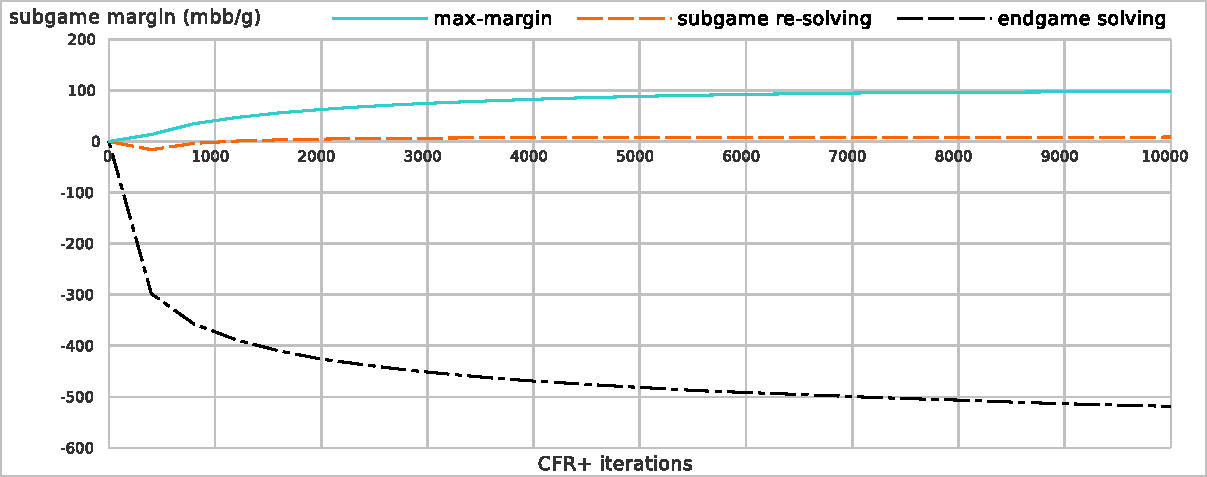
\includegraphics[width=\textwidth]{../img/sm-experiments}
  \def\captionTitle{\cfrplus iterations versus \acrshort{sm} of~refined strategies}
  \caption[\captionTitle]{\captionTitle (in milli big blinds per game).
    One big blind corresponds to 100 chips.
    The max-margin technique produces the optimal value, much greater than ones produced by~subgame re-solving or endgame solving (which has even negative \acrshort{sm}s).
    The $95\%$ confidence intervals after $10000$ iterations:
    max-margin $101.49 \pm 7.09$, subgame re-solving $8.79 \pm 2.45$, endgame solving $-518.5 \pm 49.19$
  }
  \label{fig:sm-experiments}
\end{figure}
